\section{Background}
\label{background}

The world wide web was invented 

\hl{in the beginning there was only html (no css)}

The original intent behind the web was to share documents written in HTML, CSS that used JavaScript for simple tasks such as client-side form validation \parencite{Zakai2018,Moller2018}. The set of original web technologies was all introduced in just a few years in 1993 to 1996 as illustrated in Figure \ref{figure:webtechnologies-timeline}.

\hl{more text about the figure}

% The last few years more advanced applications has moved to the web, mandating higher performance (REF).

% vi behöver ett kapitel som förklarar vad grunden ligger till problemen med benchmarking...
% dynamiska webbsidor typ som första kapitel och att de i många fall lider av prestandaproblem, sätter upp varför vi behöver benchmarking.

\begin{figure}[!h]
\centering
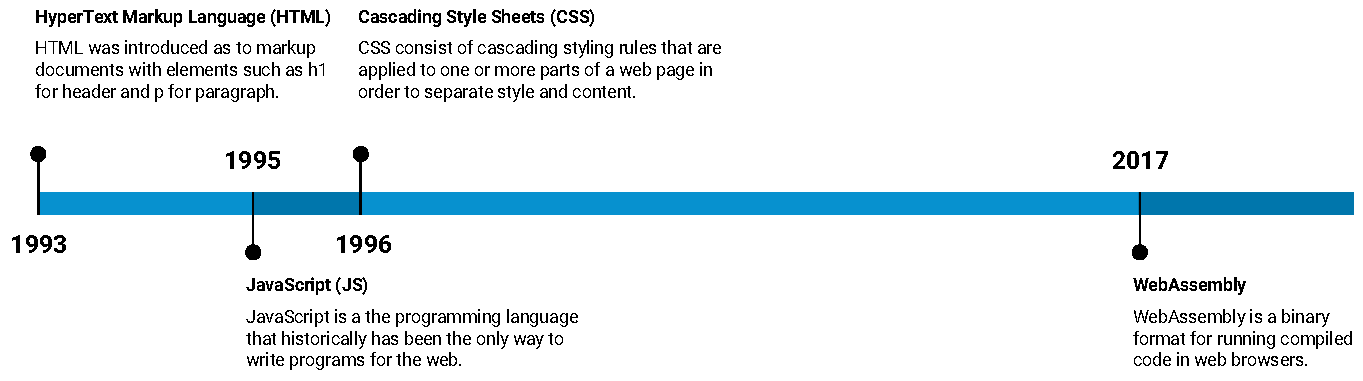
\includegraphics[width=16cm,keepaspectratio]{../Figures/webtechnologies-timeline}
\caption{Timeline of major web technologies: HTML, CSS, JavaScript and it's newest member WebAssembly.}
\label{figure:webtechnologies-timeline}
\end{figure}

\subsection{Web apps}
\subfile{webapps}

\subsection{JavaScript}
\subfile{javascript}

\subsection{WebAssembly}
\subfile{webassembly}

\subsection{Benchmarking}
\subfile{benchmarking}
